\chapter{Análisis y diseño}
\label{chap:analisis_diseño}

\lettrine{E}{n} este capítulo se expone brevemente el análisis de requisitos que se ha realizado, así como las decisiones tomadas durante el diseño.

\section{Requisitos hardware}
\label{sec:requisitos_hardware}
En esta sección se analizan los requisitos hardware (esto es, la parte tangible) del trabajo a desarrollar. Además de los tradicionales requisitos funcionales y no funcionales, se ha añadido también una sección dedicada a los denominados ``requisitos físicos'' del proyecto, ya que el aspecto físico, así como las dimensiones del mismo son un aspecto muy importante a considerar.

\subsection{Requisitos físicos}
Primeramente conviene recordar que este trabajo se lleva a cabo durante la pandemia causada por el COVID-19, por lo que la movilidad es reducida y el teletrabajo desde el domicilio la regla. Bajo estas circunstancias se comienza a realizar un diseño que satisfaga los siguientes requisitos:
\begin{itemize}
    \item El clúster debe ser \textbf{pequeño} y \textbf{manejable}: Debido a que el trabajo se realiza desde casa, éste no puede ser muy extenso, ya que el espacio es muy limitado, por lo que se deben descartar estructuras donde los nodos quedan ``libres'' y ``desperdigados'' encima de una gran mesa.
    \item El clúster debe ser \textbf{visualmente agradable} y \textbf{comprensible}: Debido a que va a ser visto por personas con (posiblemente) escasa formación en \acrshort{hpc}, el clúster ha de tener partes fácilmente identificables, lo más aisladas y señalables posible, y sobre todo no debe abrumar a quien lo ve por primera vez, esto es, no debe sentir que lo que está viendo es ``un montón de cachibaches con cables''.
\end{itemize}

\subsection{Requisitos funcionales}
En cuanto a los requisitos funcionales, como este proyecto se centra más en la divulgación que en la búsqueda de la máxima eficiencia, no se tienen unos requisitos funcionales difíciles de satisfacer. \textit{Grosso modo} se identifican:

\begin{itemize}
    \item En el clúster todos los nodos deben estar conectados entre sí en una topología \textbf{N a N}, es decir, la típica de un switch Ethernet.
    \item El clúster debe ser capaz de ejecutar aplicaciones \textbf{\acrshort{mpi}} genéricas, y en particular los \acrlong{npb}\footnote{\url{https://www.nas.nasa.gov/software/npb.html}}.
\end{itemize}

\subsection{Requisitos no funcionales}
En cuanto al resto de requisitos no funcionales, principalmente destacar que:
\begin{itemize}
    \item El clúster debe ser \textbf{sensato}: se debe emplear una calidad y cantidad de materiales adecuada a las expectativas del mismo. Esto es que, por ejemplo, el switch no debería ser el componente más caro de todo el presupuesto, pero tampoco debemos escatimar en él para aprovechar la tarjeta de red Gigabit Ethernet de las Raspberry Pi 4B.
    \item Enlazando con el requisito superior, los componentes a emplear serán actuales y aportarán una relación \textbf{calidad/precio} lo más \textbf{elevada} posible.
    \item El clúster debe ser \textbf{extensible} y \textbf{mantenible}: el despliegue hardware debe permitir modificaciones y mantenimientos de forma moderadamente sencilla.
\end{itemize}

\section{Diseño hardware}
\label{sec:diseño_hardware}
La etapa de diseño ha consumido una cantidad de tiempo para nada desdeñable, ya que diseñar un sistema que cumpla todos los requisitos no es una labor precisamente trivial. A continuación se exponen los elementos que conforman el ensamblaje del sistema, así como esquemas que documentan el diseño del mismo.

\subsection{Elementos hardware}

%%% TODO María comenta "Quedaría bien una figura compuesta de fotos de los diferentes elementos. Las fotos las podrías sacar de amazon"

En cuanto a los elementos que conforman Clúpiter, éste se compone de:
\begin{itemize}
    \item 8x Raspberry Pi 4B
    \item 8x MicroSD 32GB
    \item 1x Switch 8 puertos
    \item 1x Tarjeta de red USB 3.0 a Gigabit Ethernet 
    \item 2x Torres de \acrshort{rpi}
    \item 1x Ventilador de 120mm
    \item 1x DC-DC Step-Up Variable 
    \item 1x Fuente de alimentación 5V 150W
    \item 8x Cables USB Type-C
    \item 8x Latiguillos Ethernet
\end{itemize}

A continuación se da una explicación detallada de la decisión de estos materiales.

\subsubsection{Raspberry Pi 4B}
Este mini-computador, como se comenta previamente en \ref{sec:raspberry_pi_4_model_b}, destaca por su reducido formato de forma (del tamaño de una tarjeta de crédito), así como por su bajo consumo y coste. Esto lo hace una solución idónea para este proyecto, que no requiere de hardware muy potente, sino más bien de mucho hardware poco potente que permita simular la estructura de un supercomputador.

\subsubsection{MicroSD}
Una parte que puede pasar desapercibida en una primera aproximación, pero que es muy importante, son las tarjetas MicroSD, ya que sin ellas las Raspberry Pis no podrán arrancar ningún sistema operativo.\footnote{Desde la versión 2020-09-14 del bootloader se permite el arranque desde dispositivos USB \cite{rpibootloader20200903}}

Se han elegido las tarjetas Samsung Pro Endurance debido a su alta capacidad de escritura, ya que otros tipos de tarjetas sin este propósito específico podrían sufrir bastante desgaste y llegar al final de su vida útil prematuramente. 

La elección de la versión de 32GB de capacidad, a pesar de que no sean necesarios, es trivial, ya que no existen modelos de la misma línea de menor capacidad, y este extra de espacio puede ser bienvenido en hipotéticas futuras iteraciones sobre esta infraestructura.

%% TODO INSERTAR IMAGEN

\subsubsection{Switch Gigabit de 8 puertos}
Una de las partes más interesantes, y a las que más vueltas se le ha dado, es cómo hacer para conectar los mini computadores sin que se convierta en un lío de cables y sin que el hardware esté desproporcionado. Primeramente conviene destacar que el switch debe funcionar a 5V para poder ser alimentado directamente por la fuente de alimentación, siendo esto un importante requerimiento.
Por otro lado, también debe tenerse en cuenta que normalmente los switches se fabrican con puertos múltiplos de dos. Aunque esto pueda no parecer un problema (hay 8 dispositivos a conectar, por lo que switch de 8 puertos parece una buena opción), es conveniente tener en cuenta que el clúster debe poder ser accedido desde el exterior, lo que hace necesario un switch de 9 puertos. Estos switches, si bien existen, son escasos e innecesariamente caros, y comprar un switch de 16 puertos tampoco es una opción por las previamente mencionadas restricciones de tamaño. Para solucionar este inconveniente se añade un adaptador \nameref{sssec:usb30_gbe}.

\subsubsection{USB 3.0 a Gigabit Ethernet}
\label{sssec:usb30_gbe}
% \begin{wrapfigure}[7]{r}{0.20\textwidth}
%   \vspace*{-1.4cm}
%   \centering
%   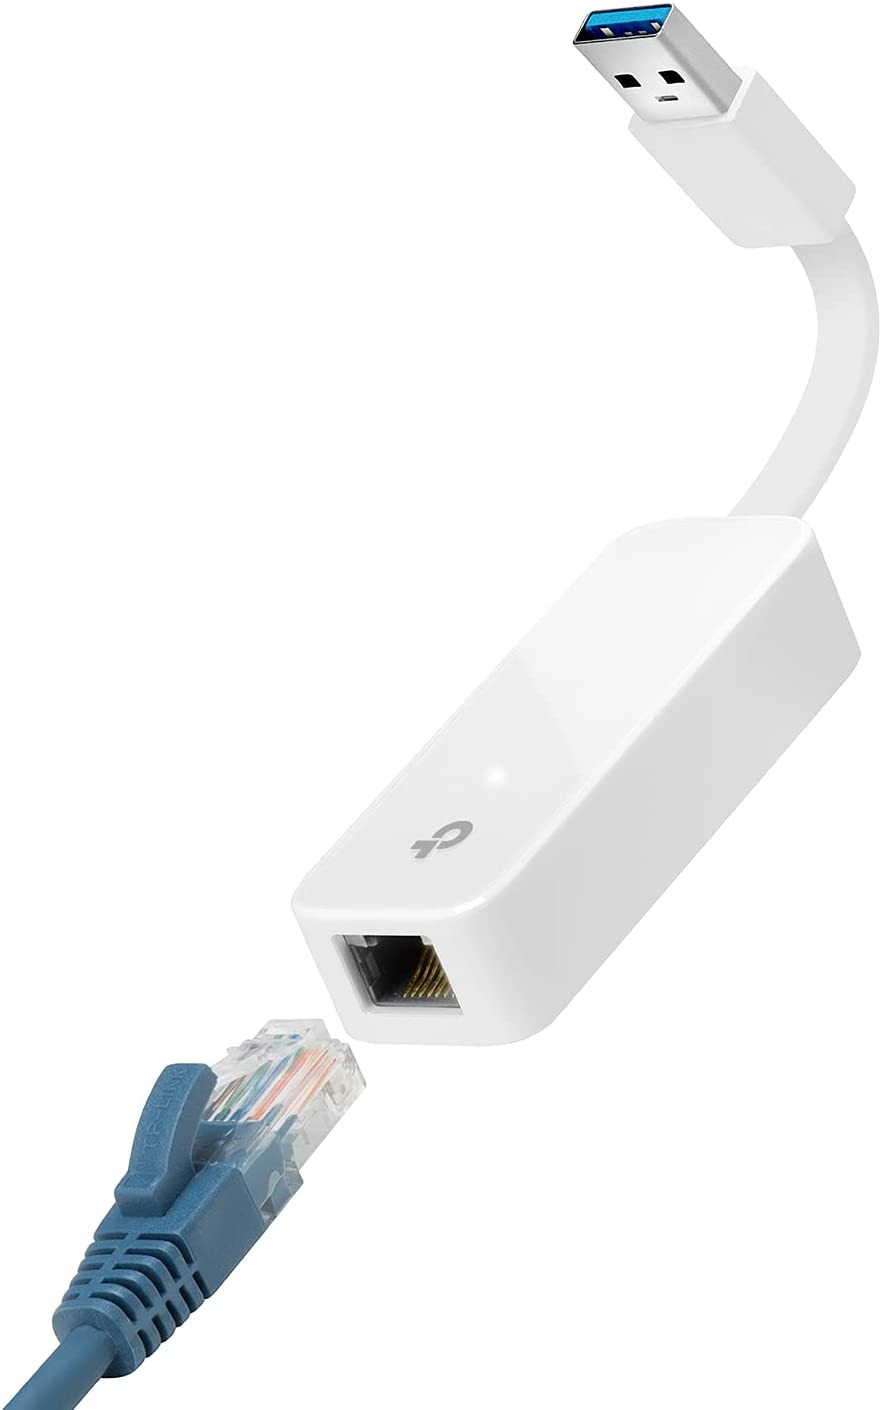
\includegraphics[width=0.20\textwidth]{img/tplink-usb-eth.jpg}
%   \label{fig:tplink-usb-eth}
% \end{wrapfigure}
Con este adaptador, y puenteando la interfaz Ethernet nativa de una Raspberry y la conectada por USB, se puede obtener virtualmente un switch de 9 puertos (Figura \ref{fig:raspi_diagram_eth}).

Esto se realiza a expensas de un pequeño coste de CPU para el manejo de los paquetes de red, que a la hora de la verdad tendrá un impacto marginal, ya que las comunicaciones intensivas se realizarán dentro del propio clúster.

\begin{figure}[h!]
  \centering
  \vspace{0.15cm}
  \def\svgwidth{0.9\textwidth}
  \input{pdf_tex/raspi_diagram_eth/raspi_diagram.pdf_tex}
  \caption{Esquema físico de red de Clúpiter}
  \label{fig:raspi_diagram_eth}
\end{figure}

\subsubsection{Torres de Raspberry Pi}
\label{sssec:torresrpi}
Las Raspberry Pis se apilan verticalmente como servidores en un rack para poder ser cableadas, accedidas, y refrigeradas de forma sencilla, además de resultar visualmente agradables en esta disposición.

% \begin{wrapfigure}[4]{r}{0.35\textwidth}
%   \vspace*{-0.3cm}
%   \centering
%   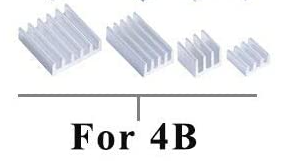
\includegraphics[width=0.35\textwidth]{img/disipadores-rpi-4b.png}
%   \label{fig:rpi4b-disipadores}
% \end{wrapfigure}
Estos kits incluyen disipadores para RAM, CPU, controlador Ethernet y USB, así como refrigeración activa, que no se instalará en este caso tal como se comenta en la siguiente subsección.



% TODO INSERTAR IMAGEN DE TORRES Y DISIPADORES

\subsubsection{Ventilador de 120mm}
% \begin{wrapfigure}[8]{r}{0.28\textwidth}
%   \centering
%   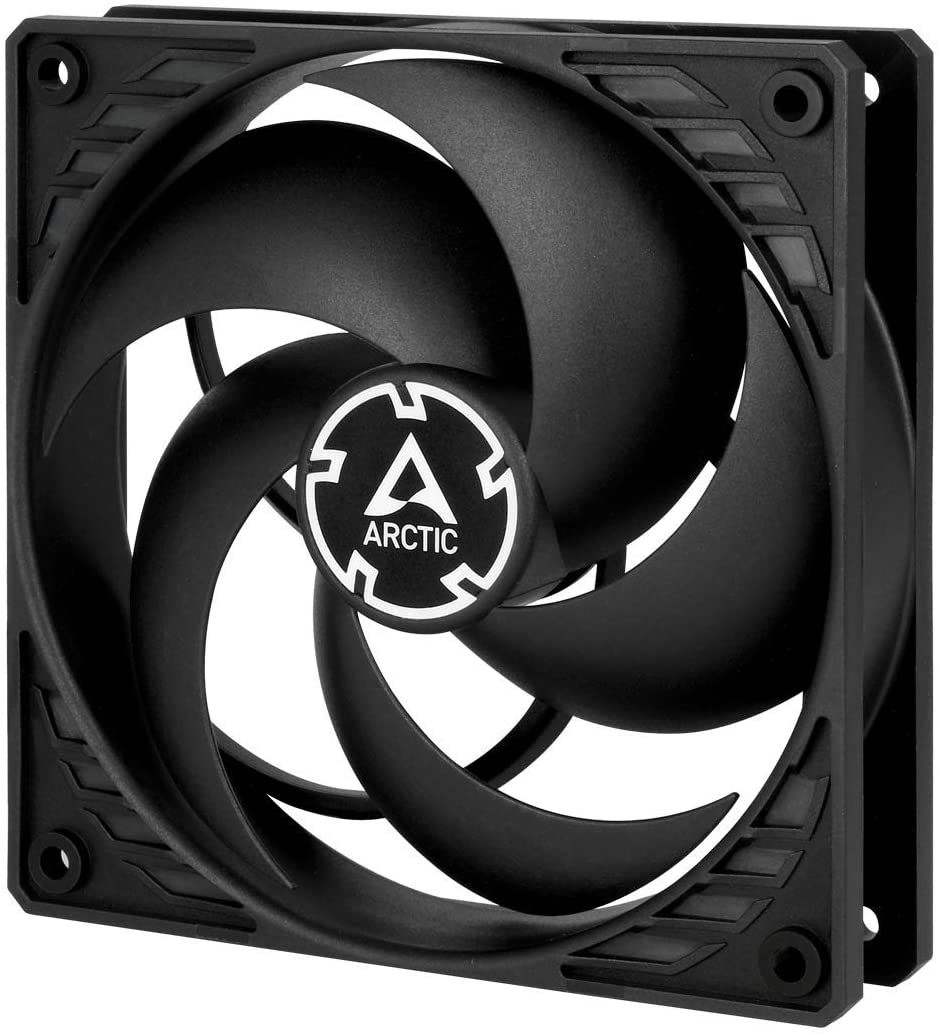
\includegraphics[width=0.28\textwidth]{img/arctic-fan.jpg}
%   \label{fig:arctic-fan}
% \end{wrapfigure}
Como se menciona previamente, las \nameref{sssec:torresrpi} incluyen refrigeración activa, pero se ha optado por no incluirla por el nivel de ruido que hacen, a parte de la poca necesidad de la misma dada la naturaleza del proyecto. Sin embargo, para permitir la extensibilidad del proyecto en forma de nuevas iteraciones, se ha añadido un ventilador de 120mm optimizado para presión, que mueve aire de un extremo al otro del clúster, refrigerando los mini computadores con ayuda de los disipadores instalados.

Volviendo a hablar de tensiones, el ventilador elegido funciona a 12V. Sin embargo, alimentarlo a esa tensión haría que funcionase a máxima potencia constantemente. Para evitar esto, los fabricantes de ventiladores utilizan principalmente dos aproximaciones: regulación de voltaje y modulación por ancho de pulsos, o \acrshort{pwm}. Esta regulación de voltaje se realiza informada por la línea de tacómetro, sin embargo, en este caso, dados los requerimientos térmicos de los mini computadores empleados, únicamente se empleará un step-up variable\footnote{Con step-up variable entendemos un circuito que, dada una tensión de entrada, puede ajustarse una tensión de salida igual o superior a la de la entrada en función del valor de la resistencia de un potenciómetro} MT3608 con el que se mantiene el ventilador a una velocidad fija (y lo más baja posible para rebajar el nivel de ruido), ignorando la línea de tacómetro.
% \hfill\ \ \begin{wrapfigure}[4]{l}{0.28\textwidth}
%   %\vspace*{-1cm}
%   \centering
%   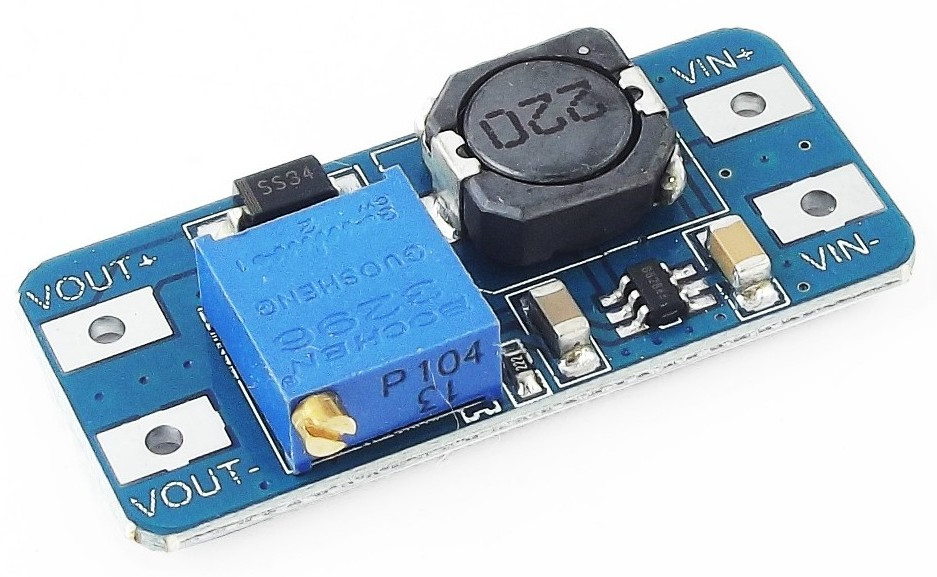
\includegraphics[width=0.28\textwidth]{img/step-up.jpg}
%   \label{fig:step-up}
% \end{wrapfigure}
De esta forma el usuario tiene la posibilidad de elevar la potencia en el improbable escenario de que se necesitase más caudal de aire. Esto ocurriría principalmente si en otra iteración sobre este trabajo se decide hacer \gls{overclock} a los nodos.

\subsubsection{Fuente de alimentación 5V 150W}
La fuente de alimentación es un componente fundamental del clúster, y es que las Raspberry Pi 4 consumen una cantidad de energía baja, pero tampoco tan baja como se podría imaginar. Solamente el propio dispositivo funcionando a pleno rendimiento consume alrededor de 7.5W, consumo que se dispara si se enchufan periféricos a sus puertos USB. Por esta razón la Raspberry Pi foundation, en lo que debe ser un movimiento para ahorrar problemas a usuarios menos experimentados, recomienda 3A (a 5V) por Raspberry Pi, es decir, 15W por dispositivo \cite{raspberrypi_power-requirements}.

\begin{figure}[h!]
  \vspace*{0.5cm}
  \centering
  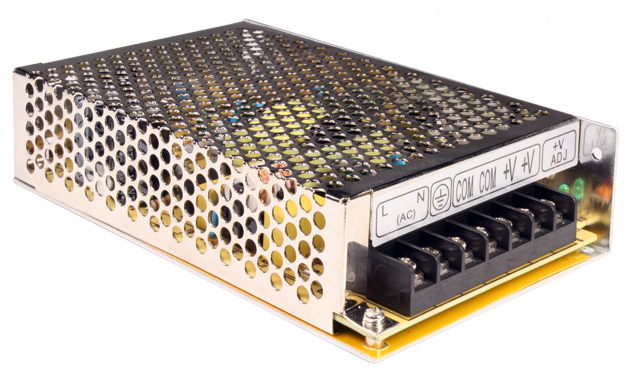
\includegraphics[width=0.60\textwidth]{img/psu.jpg}
  \caption{Fuente de Alimentación AC-DC SA5C150W5}
  \label{fig:psu_photo}
  \vspace*{0.1cm}
\end{figure}

Dadas estas circunstancias, y para ahorrar posibles problemas presentes y futuros, se ha optado por una fuente de alimentación AC-DC de 5V con una potencia de 150W, modelo SA5C150W5 (Figura \ref{fig:psu_photo}), que sin duda satisface por más del doble los requerimientos energéticos de Clúpiter en su estado actual. La conexión eléctrica de todos los componentes discutidos previamente se puede observar en la Figura \ref{fig:raspi_electric_diagram}.

\begin{figure}[h!]
  \centering
  \vspace*{0.5cm}
  \def\svgwidth{0.9\textwidth}
  \input{pdf_tex/electric_diagram/electric_diagram.pdf_tex}
  \caption{Diagrama eléctrico de Clúpiter}
  \label{fig:raspi_electric_diagram}
\end{figure}

\subsubsection{Cableado eléctrico y de red}
\label{sssec:cableado_electrico_red}
% \begin{wrapfigure}[6]{r}{0.125\textwidth}
%   \centering
%   \vspace*{-1.25cm}
%   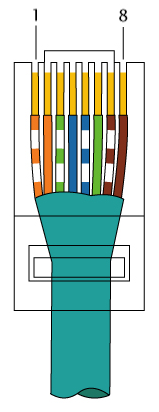
\includegraphics[width=0.125\textwidth]{img/TIA-568B.png}
%   \label{fig:TIA-568B}
% \end{wrapfigure}
Tras la lista de componentes previamente expuestos, únicamente queda tratar la interconexión de los mismos, un componente que ha dado más problemas de lo que pueda parecer.

En cuanto al cableado Ethernet no hay mucho que clarificar. Los cables de 4 pares trenzados Cat5E se cortan a la longitud necesaria, y se crimpan siguiendo la disposición ANSI/TIA-568B (Figura \ref{fig:TIA-568B-horiz}).

\begin{figure}[h!]
  \centering
  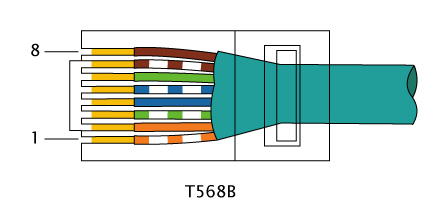
\includegraphics[width=0.55\textwidth]{img/TIA-568B-horizontal.png}
  \caption{Cable Ethernet según disposición ANSI/TIA-568B}
  \label{fig:TIA-568B-horiz}
\end{figure}

El cableado eléctrico ha creado importantes problemas, y es que las Raspberry Pi 4 Model B son alimentadas por USB Tipo-C, teniendo una implementación del mismo un tanto particular, por lo que no cualquier cable funciona como podría esperarse. Esto provocó el tener que cambiar los cables originalmente planeados.

En un principio se realizó la compra de 4 cables terminados en USB-C en cada extremo, por lo que al cortarlos por la mitad se podrían obtener 8 cables terminados en USB-C. El principial problema con esta compra es que entregar potencia a través del USB-C tiene su propia especificación, USB Power Delivery (USB-PD). Tras descubrir este detalle después de la compra del material, y tras ver que realizando el arreglo (Figura \ref{fig:usb_pd_schematic} \cite{usb_pd_techforum}), que no resultaría ni caro ni complicado, aún existía la probabilidad de que (debido a la no-estándar implementación de USB-C en este modelo de Raspberry Pi) la entrega de potencia siguiese sin funcionar, se decidió por no seguir por esa vía, y realizar la compra de 8 cables con experiencia positiva previa de otros usuarios.

\begin{figure}[h!]
  \vspace*{0.5cm}
  \centering
  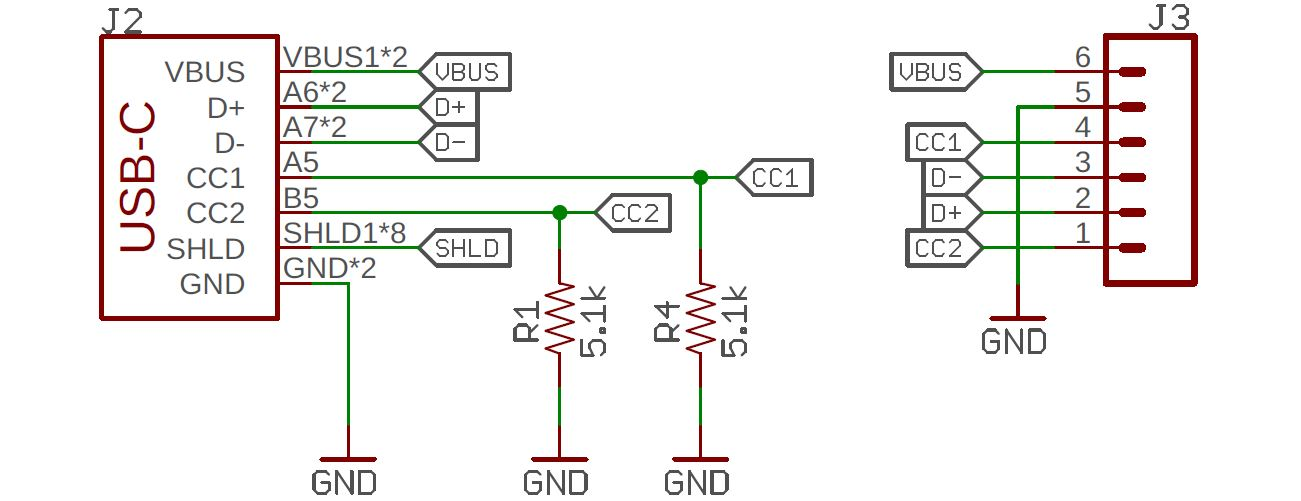
\includegraphics[width=0.8\textwidth]{img/usb_pd_schematic.jpg}
  \caption{Esquemático para USB-C Power Delivery 5V y 3A}
  \label{fig:usb_pd_schematic}
  \vspace*{0.1cm}
\end{figure}

Este nuevo (y el actual) cableado eléctrico es un cable USB-C con terminación magnética y que soporta una corriente de 3A a 5V. Esto permite abstraer los detalles de implementación a nivel eléctrico del USB Tipo-C y expone simplemente los cables de +5V y masa.

Un aspecto muy importante a tener en cuenta, y que ha sido un problema de relevancia durante la construcción del clúster, es que debido a la naturaleza de estos cables, el contacto entre la pieza del USB-C y el propio cable debe estar limpio de residuos aislantes o conductores de un diámetro lo suficientemente grande que impidan un buen contacto.

Otra opción que se barajó pero se terminó descartando fue la alimentación directa por los pines +5V y GND del \acrshort{gpio}, pero que se terminó descartando porque realizar la alimentación salta por completo todo el sistema de protección, lo cual podría resultar fatal en caso de fallo en la fuente de alimentación.

% TODO INSERTAR IMAGENES CABLES USB INALAMBRICOS Y ANSI-TIA
% TODO INSERTAR IMAGENES DE PIEZAS


\subsection{Diseño estructural}
\label{ssec:diseño_estructural}
La estructura que se ha pensado para aprovechar el espacio lo máximo posible consiste en lo que podría llamarse coloquialmente ``un sandwich'': la fuente de alimentación en la parte baja; las Raspberry Pi en la zona intermedia, siendo refrigeradas por un ventilador posicionado verticalmente; y el switch en la parte alta, creando cierto encajonamiento al más puro estilo supercomputador, como se muestra en la Figura \ref{fig:render_cluster_1}.

\begin{figure}[h!]
  \centering
  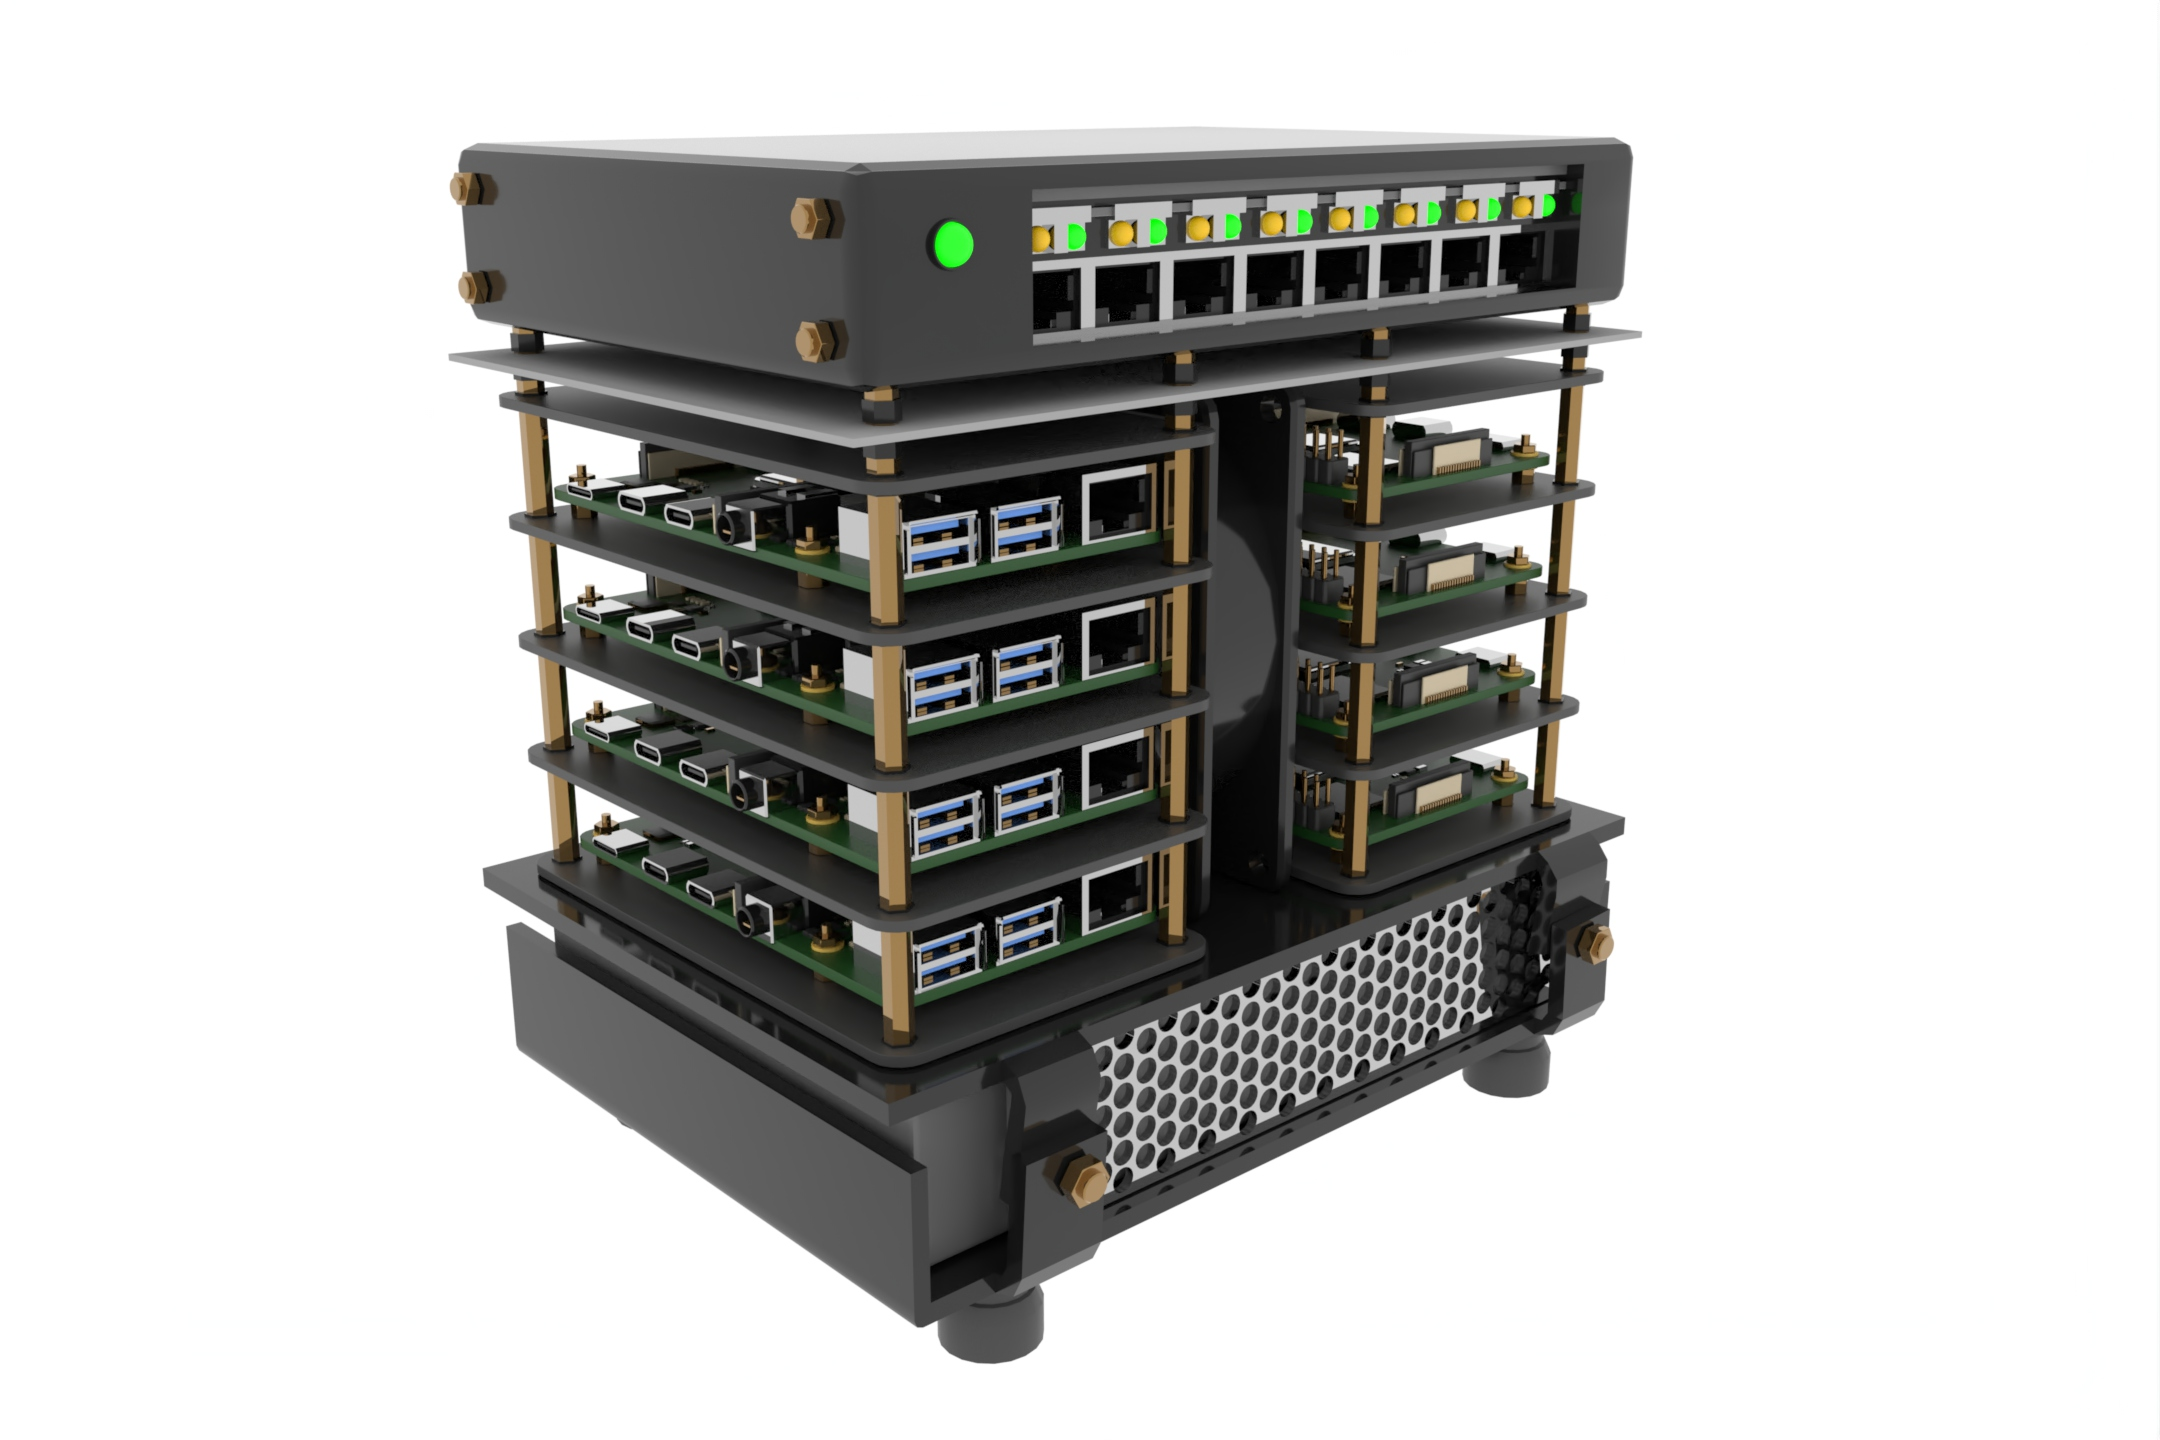
\includegraphics[width=\textwidth]{img/cluster_render_front.jpg}
  \caption{Render frontal del clúster}
  \label{fig:render_cluster_1}
\end{figure}

El acoplamiento entre las capas se realiza mediante láminas de chapa, en las que se atornillan las piezas de arriba y de abajo, sirviendo como adaptador.

% TODO QUIZÁS PONER QUE SE ANEXAN PLANOS CAD?

\section{Requisitos software}
\label{sec:requisitos_software}
En esta sección se analizan los requisitos software del proyecto. Para el desarrollo del mismo necesitamos dos piezas de software clave: el sistema operativo, y la aplicación web.

Como se comenta en \nameref{sec:objetivos}, se utilizará Arch Linux como distribución Linux. Esto es así porque siendo un usuario con cierta experiencia, resulta extremadamente cómodo instalar un sistema mínimo basado en esta distribución, así como mantenerlo y ampliarlo, cumpliendo el requisito de extensibilidad del hardware, que también aplica al software. Además, a un hipotético usuario futuro sin tanta experiencia le resultará sencillo habituarse al funcionamiento y configuración de Arch Linux debido a su amplia documentación en la Arch Wiki.\footnote{\url{https://wiki.archlinux.org}. Se puede consultar una breve guía de mantenimiento básico de Arch Linux en el Apéndice \ref{chap:archlinux_maintenance_guide}}

Por otro lado, se implementará una aplicación web (\textit{dashboard}) que permita:
\begin{enumerate}
    \item \textbf{Explicar el funcionamiento} de Clúpiter, los supercomputadores paralelos, \acrshort{mpi}, y la importancia en el mundo real de los mismos, mediante vídeos reproducibles en la página web.
    \item \textbf{Monitorizar el estado} e histórico del servidor en tiempo real, pudiendo realizar con la ayuda de dicha información explicaciones interactivas acerca del funcionamiento de programas \acrshort{mpi}.
\end{enumerate}

Como principal requisito no funcional, y como ya se menciona previamente:
\begin{itemize}
    \item El sistema operativo de Clúpiter debe ser \textbf{extensible} y \textbf{mantenible}. El sistema operativo no debe ser una caja negra inaccesible y difícil de mantener, sino todo lo contrario.
\end{itemize}

\section{Diseño software}
En esta sección se describen las decisiones de diseño del software de Clúpiter, así como todo lo que no sea hardware propiamente dicho, esto es, por ejemplo, el direccionamiento lógico de red.

\subsection{Dashboard}
La funcionalidad discutida en el apartado anterior se proporcionará mediante el uso de la tecnología de WebSockets\footnote{\url{https://socket.io}} y Netdata\footnote{\url{https://www.netdata.cloud}}. La implementación del dashboard haciendo uso de estas tecnologías se describe en detalle en el Capítulo \ref{chap:aplicacion_web}, Sección \ref{sec:contenido_didactico__diseño}.

\subsection{Diseño lógico de red}
A nivel lógico, la asignación de direcciones IP es muy sencilla. Se opta por la asignación estática de IPs del rango 192.168.0.22X, siendo X el número de la \acrlong{rpi}, del 0 al 7.

Además, la puerta de enlace será fija en la dirección 192.168.0.1, pudiendo estar esta presente o no. Esto abre la puerta a tres escenarios:
\begin{itemize}
    \item Clúpiter puede ser conectado a un switch que da acceso a una red con puerta de enlace en la dirección 192.168.0.1, y así tener acceso a internet.
    \item Clúpiter puede ser conectado directamente a un ordenador que hace routing, y se asigna en el segmento de red interna del clúster, la IP de gateway, permitiendo también acceso a internet.
    \item Un ordenador se conecta directamente a Clúpiter, con cualquier IP que no esté en conflicto, y puede realizar SSH a cualquier nodo y acceder a todas sus funciones, pero los nodos del clúster no tendrán acceso a internet.
\end{itemize}

Esto es posible debido a que virtualmente Clúpiter está conectado a un switch de 9 puertos, como se puede observar en la Figura \ref{fig:raspi_diagram_eth}: \nameref{fig:raspi_diagram_eth}. El esquema lógico de red para el caso en el que existe un host conectado al clúster, en la IP 192.168.0.1, haga de gateway o no (en el diagrama sí es el gateway), se puede ver en la Figura \ref{fig:raspi_diagram_logical}.

\begin{figure}[h!]
  \centering
  \vspace*{0.5cm}
  %\def\svgwidth{0.87\textwidth}
  \def\svgwidth{0.9\textwidth}
  \input{pdf_tex/raspi_logical_net/raspi_logical_net.pdf_tex}
  \caption{Esquema lógico de red de Clúpiter}
  \label{fig:raspi_diagram_logical}
\end{figure}